% Created 2017-02-22 Wed 08:33
\documentclass[11pt]{article}
\usepackage[utf8]{inputenc}
\usepackage[T1]{fontenc}
\usepackage{fixltx2e}
\usepackage{graphicx}
\usepackage{longtable}
\usepackage{float}
\usepackage{wrapfig}
\usepackage{rotating}
\usepackage[normalem]{ulem}
\usepackage{amsmath}
\usepackage{textcomp}
\usepackage{marvosym}
\usepackage{wasysym}
\usepackage{amssymb}
\usepackage{hyperref}
\tolerance=1000
\date{Feb 20-24, 2017}
\title{Week 6 lecture notes - PSYC 3435}
\hypersetup{
  pdfkeywords={},
  pdfsubject={},
  pdfcreator={Emacs 25.1.1 (Org mode 8.2.10)}}
\begin{document}

\maketitle
Any experimental design comes down to knowing two things:
\begin{itemize}
\item dependent variables: what is measured
\item independent variables: what is manipulated
\end{itemize}

\section*{Dependent variables}
\label{sec-1}

Need to consider the following:
\begin{itemize}
\item how things are measured (scale of measurement)
\item whether measure is valid
\item whether measure is reliable
\end{itemize}

\subsection*{Scales of measurement}
\label{sec-1-1}
\begin{itemize}
\item nominal: non-ordered, categorical responses (e.g., gender, college major)
\item ordinal: ordered, categorical responses (e.g., level of anxiety, rating how "often" something occurs)
\item interval: numerical responses with no meaningful "0" (e.g., Likert scales)
\item ratio: numerical responses with a "0" (so ratios make sense) (e.g., RT, temperature)
\item Note -- type of scale determines statistical test that can be used!
\end{itemize}

\subsection*{Validity - how accurate is your measurement?}
\label{sec-1-2}
\begin{itemize}
\item usually an issue with surveys
\item construct validity - extent to which survey measures what is intended to
\item face validity - on the surface, survey appears to be a good measure
\end{itemize}

\subsection*{Reliability - how consistent is your measurement}
\label{sec-1-3}
\begin{itemize}
\item test-retest reliability - extent to which survey gives same score over different administrations
\item interrater reliability - extent to which different observers rate behaviors the same
\end{itemize}

\section*{Independent variables}
\label{sec-2}

Three main ways an IV can be manipulated:
\begin{enumerate}
\item Presence/absence - a treatment is either present or absent (2 levels)
\item Type - each level of IV involves a different type of treatment (e.g., type of instruction on a test)
\item Amount - each level varies the amount of something (e.g., drug dosage)
\end{enumerate}

\section*{Internal validity and bias}
\label{sec-3}
Recall that internal validity refers to the extent to which an experiment provides inference for causation.
Let's look at one example of a study with LOW internal validity:

\subsection*{class demo: a "test of attentional focus"}
\label{sec-3-1}

\begin{enumerate}
\item divide room into two groups (male and female is best)
\item Females given Stroop task with no interference\ldots{}measure time
\end{enumerate}
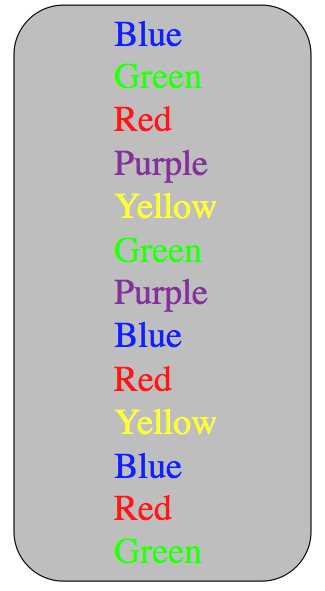
\includegraphics[width=.9\linewidth]{figures/list1.jpg}

\begin{enumerate}
\item Males given Stroop task with interference\ldots{}measure time
\end{enumerate}

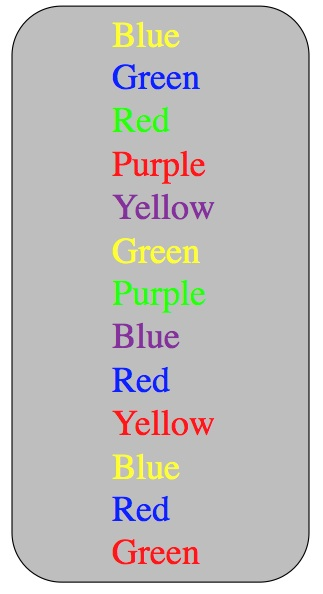
\includegraphics[width=.9\linewidth]{figures/list2.jpg}

\begin{enumerate}
\item Who wins?  Does that mean males/females have better attentional focus?
\end{enumerate}

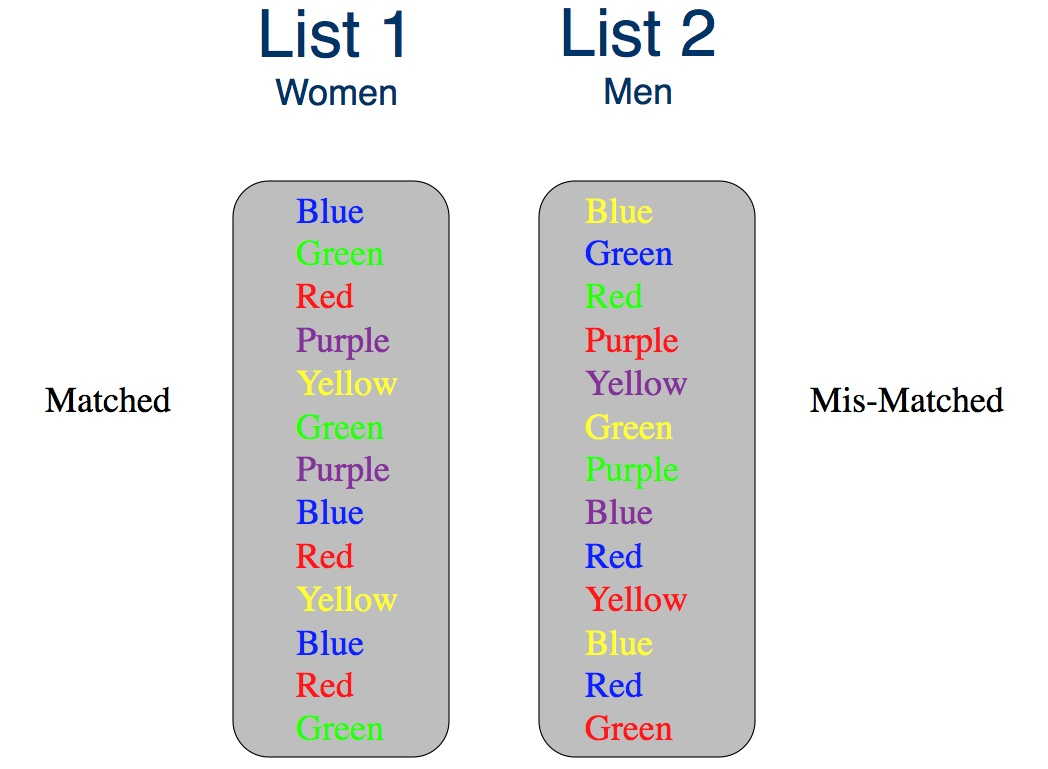
\includegraphics[width=.9\linewidth]{figures/compare.jpg}

\subsection*{Confounds}
\label{sec-3-2}

The problem with our inference in this experiment is that one variable (color/word interference) is perfectly correlated with another (gender).  This is called a \emph{confound}, and it is a threat to internal validity.

The goal in experimental design is to minimize confounds.

Types of confounds (and solutions):
\begin{itemize}
\item Group differences (solution: use random assignment)
\item Order/testing effects (solution: use counterbalancing)
\item experimenter bias (solution: use blinding)
\end{itemize}
% Emacs 25.1.1 (Org mode 8.2.10)
\end{document}